\documentclass{tufte-handout}

\title{On ultimate; O4: primary long or right-wing}
\author[James Reynolds]{James Reynolds}

%\date{28 March 2010} % without \date command, current date is supplied

%\geometry{showframe} % display margins for debugging page layout

\usepackage{graphicx} % allow embedded images
  \setkeys{Gin}{width=\linewidth,totalheight=\textheight,keepaspectratio}
  \graphicspath{{graphics/}} % set of paths to search for images
\usepackage{amsmath}  % extended mathematics
\usepackage{booktabs} % book-quality tables
\usepackage{units}    % non-stacked fractions and better unit spacing
\usepackage{multicol} % multiple column layout facilities
\usepackage{lipsum}   % filler text
\usepackage{fancyvrb} % extended verbatim environments
  \fvset{fontsize=\normalsize}% default font size for fancy-verbatim environments

% Standardize command font styles and environments
\newcommand{\doccmd}[1]{\texttt{\textbackslash#1}}% command name -- adds backslash automatically
\newcommand{\docopt}[1]{\ensuremath{\langle}\textrm{\textit{#1}}\ensuremath{\rangle}}% optional command argument
\newcommand{\docarg}[1]{\textrm{\textit{#1}}}% (required) command argument
\newcommand{\docenv}[1]{\textsf{#1}}% environment name
\newcommand{\docpkg}[1]{\texttt{#1}}% package name
\newcommand{\doccls}[1]{\texttt{#1}}% document class name
\newcommand{\docclsopt}[1]{\texttt{#1}}% document class option name
\newenvironment{docspec}{\begin{quote}\noindent}{\end{quote}}% command specification environment

\begin{document}

\maketitle% this prints the handout title, author, and date
%\printclassoptions
This is 
a two-pager 
about
primary long and 
right wing on offence\footnote{
Referred to here 
as position O4. 
This
is part of a series, 
available at
\url{https://github.com/James-Reynolds/Ultimate-strategy-and-tactics}}. 

\section{Beating person-match defence with a vertical stack}\label{sec:vertical}

\begin{marginfigure}%
  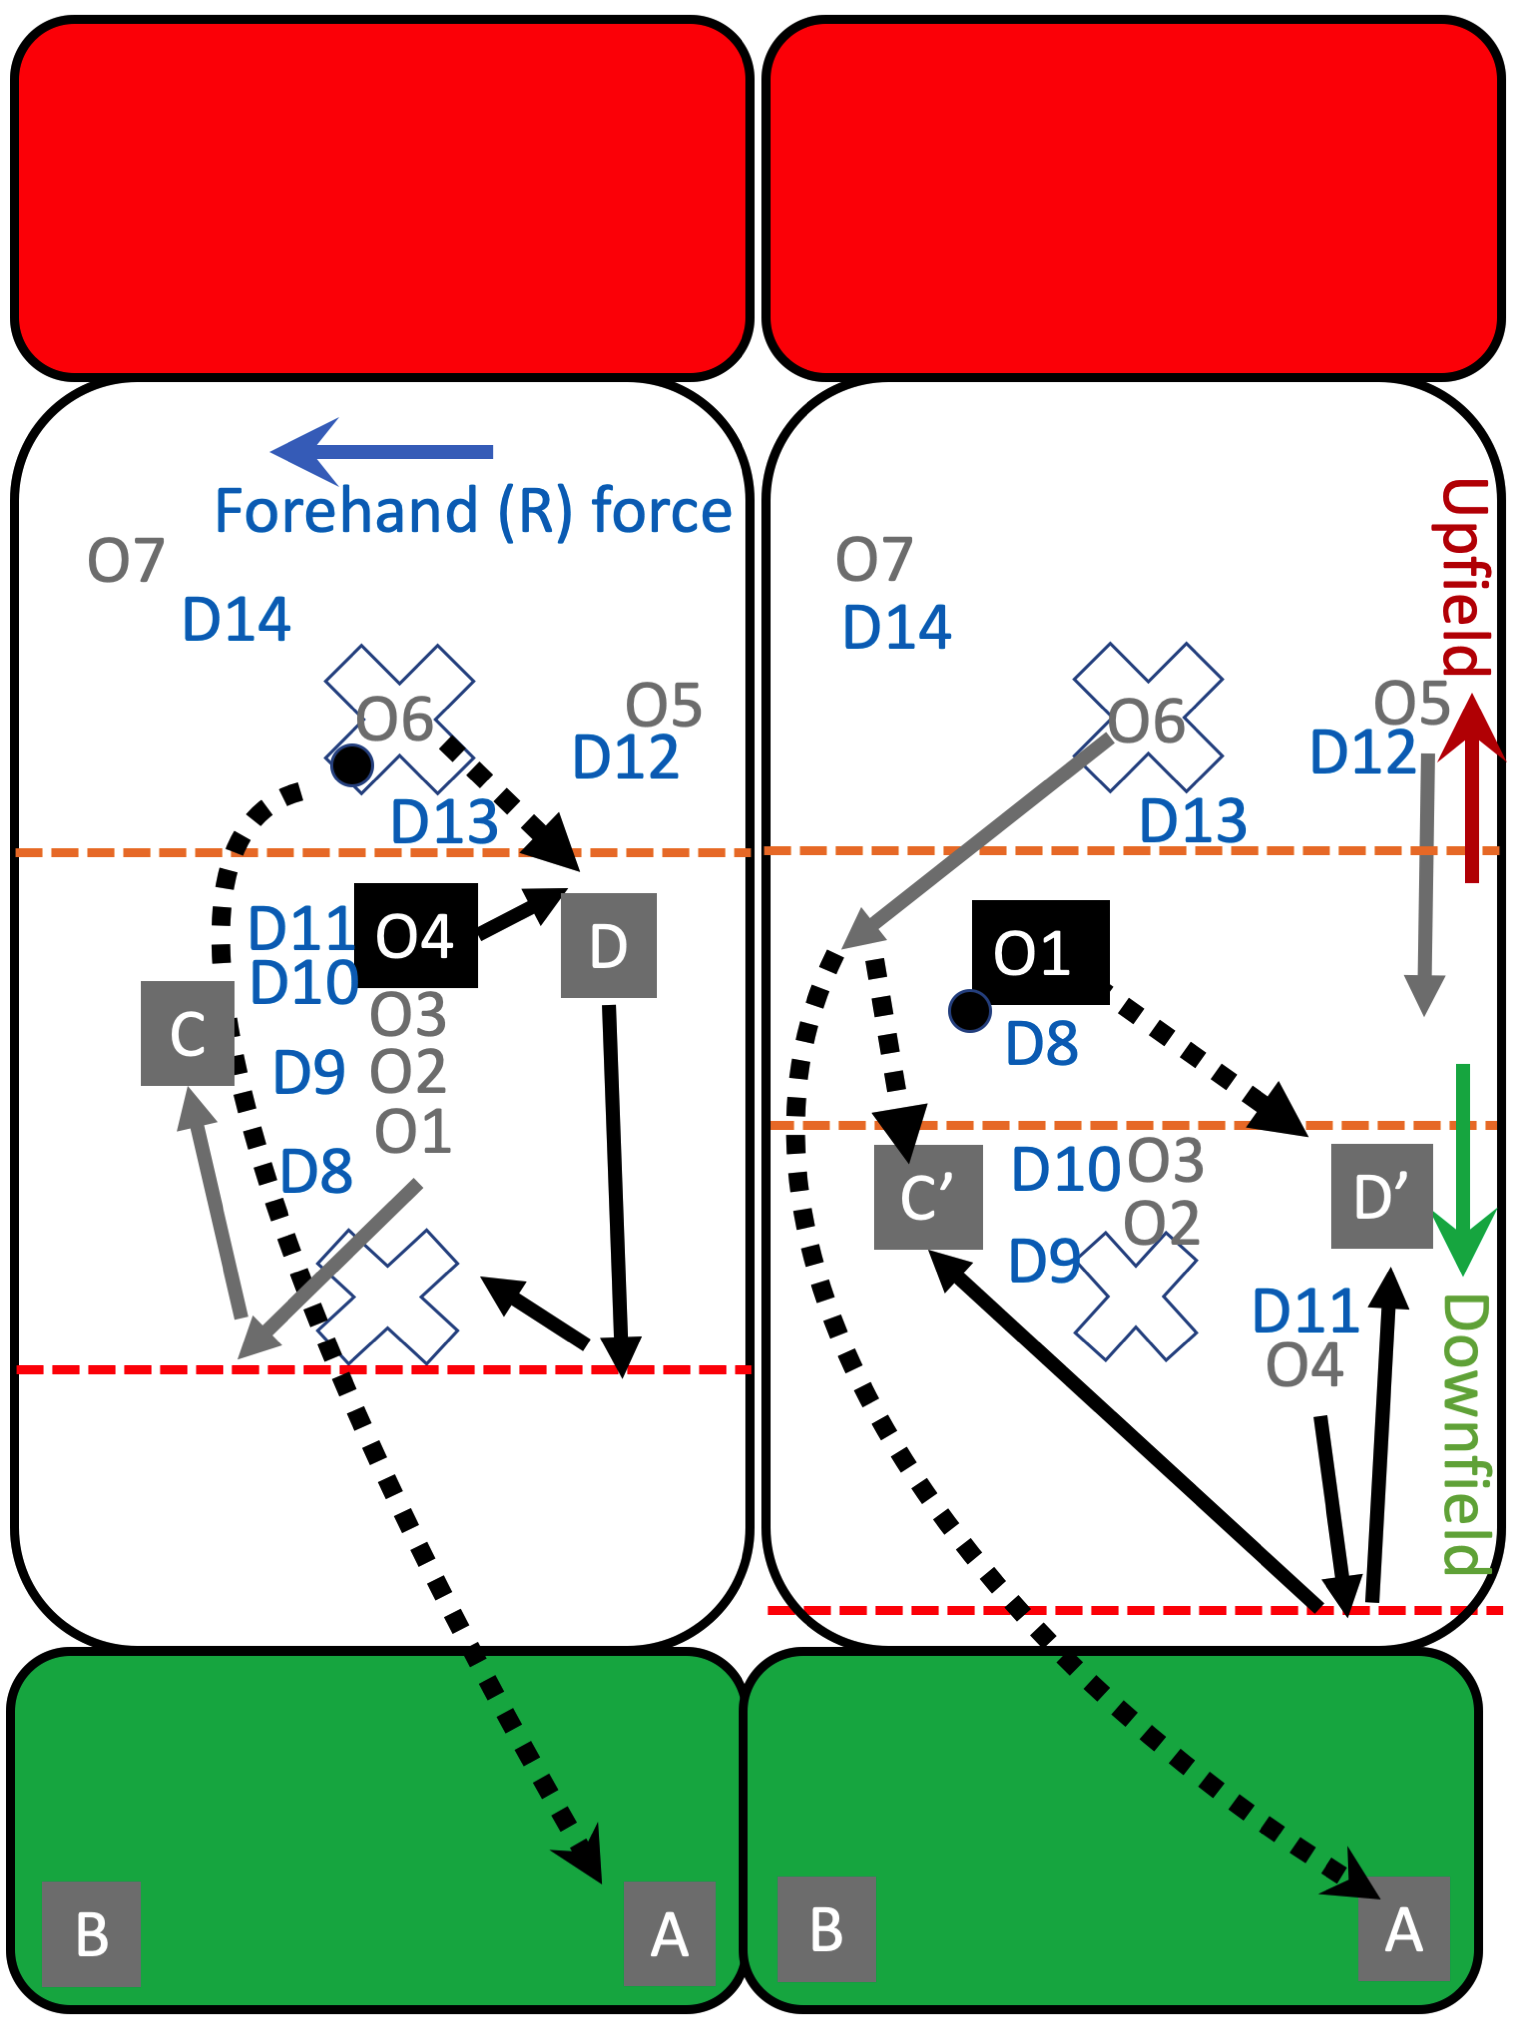
\includegraphics[width=\linewidth]{O4-vertical}
  \caption{Vertical stack: 
  starting position (left),
  D11 poaching deep (top-right) 
  and disc moved to C means D11 
  covers O4 (bottom-right)}
  \label{fig:O4-vertical}
\end{marginfigure}

Figure \ref{fig:O4-vertical} (left) shows 
your team: 
using 
a vertical stack formation; 
having called a brick; and
facing a 
forehand force with 
person-match defence\footnote{
Vertical works
against other person-match defences, 
but might need 
adjustment e.g. 
(1) backhand force,
mirror everything;
(2) straight up force, 
maybe give the handlers 
time to move the disc around, 
and go out to the sidelines
when you do cut; etc.}. 
You (O4) 
are shown 
at the front 
of the stack.
D11 
is likely to set up, 
as shown, 
to defend the open side. 
O6 might
therefore be 
able to 
throw a break-force 
you going to D\footnote{
You may
be able to stand still, 
simply wait for O6 
to throw, 
and then run onto 
it at D.}.
If you do not 
receive the disc 
at D, 
you might then 
cut downfield 
on the break side 
of the field, 
heading towards 
A\footnote{
Watch out that you 
do not cause a pick 
between D11, 
D10 and O3.}.  

The third, 
solid black arrow
shown in 
Figure \ref{fig:O4-vertical} (left) 
indicates you 
returning to 
the rear of the stack, 
or you might continue 
and cut to C. 
However, the dashed, 
red, 
horizontal line 
indicates the limit 
of how far you 
would go downfield\footnote{
The position of 
this line 
varies with movement 
of the disc and the distance 
that the person with the disc 
can (or is likely to) throw.
The dashed, 
yellow line, 
similarly indicates 
approximately the
limit of how far you 
would go upfield.  
Any further and
you are crowding the handlers, 
and your defender 
might be able to interfere 
with the dump}. 
Figure \ref{fig:O4-vertical} (top-right) shows 
what might happen 
if you go downfield of
the dashed red line 
prior to the disc being thrown. 
Because the disc travels slowly 
through the air, 
D11 will no longer has to stay as close to you 
to prevent or intercept a throw 
(to you and/or A)
D11 is therefore able to play 
further upfield 
so as to 
cover you if you 
cut back towards 
the disc. 
They might also 
poach, so as to 
potentially intercept
or prevent 
downfield throws 
to O1-3\footnote{
Note how Figure \ref{fig:O4-vertical} (top-right)  
shows D8-10 
having changed their 
positioning 
to cover O1-3
almost exclusively upfield, 
preventing the under cut.  
This is possible because you (O4) 
are so deep, 
that D8-10 may be 
able to rely on 
D11 intercepting 
or preventing any deep throws 
to their direct opponents.}. 

Figure \ref{fig:O4-vertical} (bottom-right)  
provides an example 
of a similar situation, but 
where the disc has moved 
in the meantime to O1, 
who cut to C.  
The dashed,
red,
horizontal line 
is shown 
further downfield in 
Figure \ref{fig:O4-vertical} (bottom-right), 
reflecting that if O1 
throws the disc to 
A it will arrive 
more quickly than before, 
when O6 had it further upfield. 
Hence, D11 will likely 
have to play tighter defence 
on you (O4), 
meaning that O2 and O3 
will be able to cut deep to B.

As primary long, 
your role is 
typically to provide 
a target for a scoring throw 
into the endzone, or 
otherwise gain a lot of 
territory. If you do get the disc,
you might be able to immediately
pass to one of the other cutters 
(O1-3). 
However, 
you are also cutter, 
so the most 
important things to do are:
to make sure your team 
retains possession of the disc.
Hence, 
if no (safe) pass downfield 
is immediately available, 
it is probably time to engage 
one of the handlers (O5-7), 
throw a dump, 
and get downfield again 
to do some more cutting.  
The handlers can take care
of the throwing, 
but your team likely 
needs you to be a target, 
which the handlers are likely 
too far upfield to provide.


\subsection{Beating person-match defence with feldrunner}
\label{sec:feld}
Figure \ref{fig:O4-horizontal} (left) 
shows a feldrunner formation, 
with 4 handlers (O4-7), 
and O1 as the focus.
You  
(O4) 
and O2
are in the endzone. The idea of feldrunner 
is to pass to 
the isolated
focus (O1). 
They will then either pass to 
O2 or you, 
or dump to the handlers
and reset. This formation relies 
on you and O2 
waiting until O1 
gets the disc 
before cutting.  
\begin{marginfigure}%
  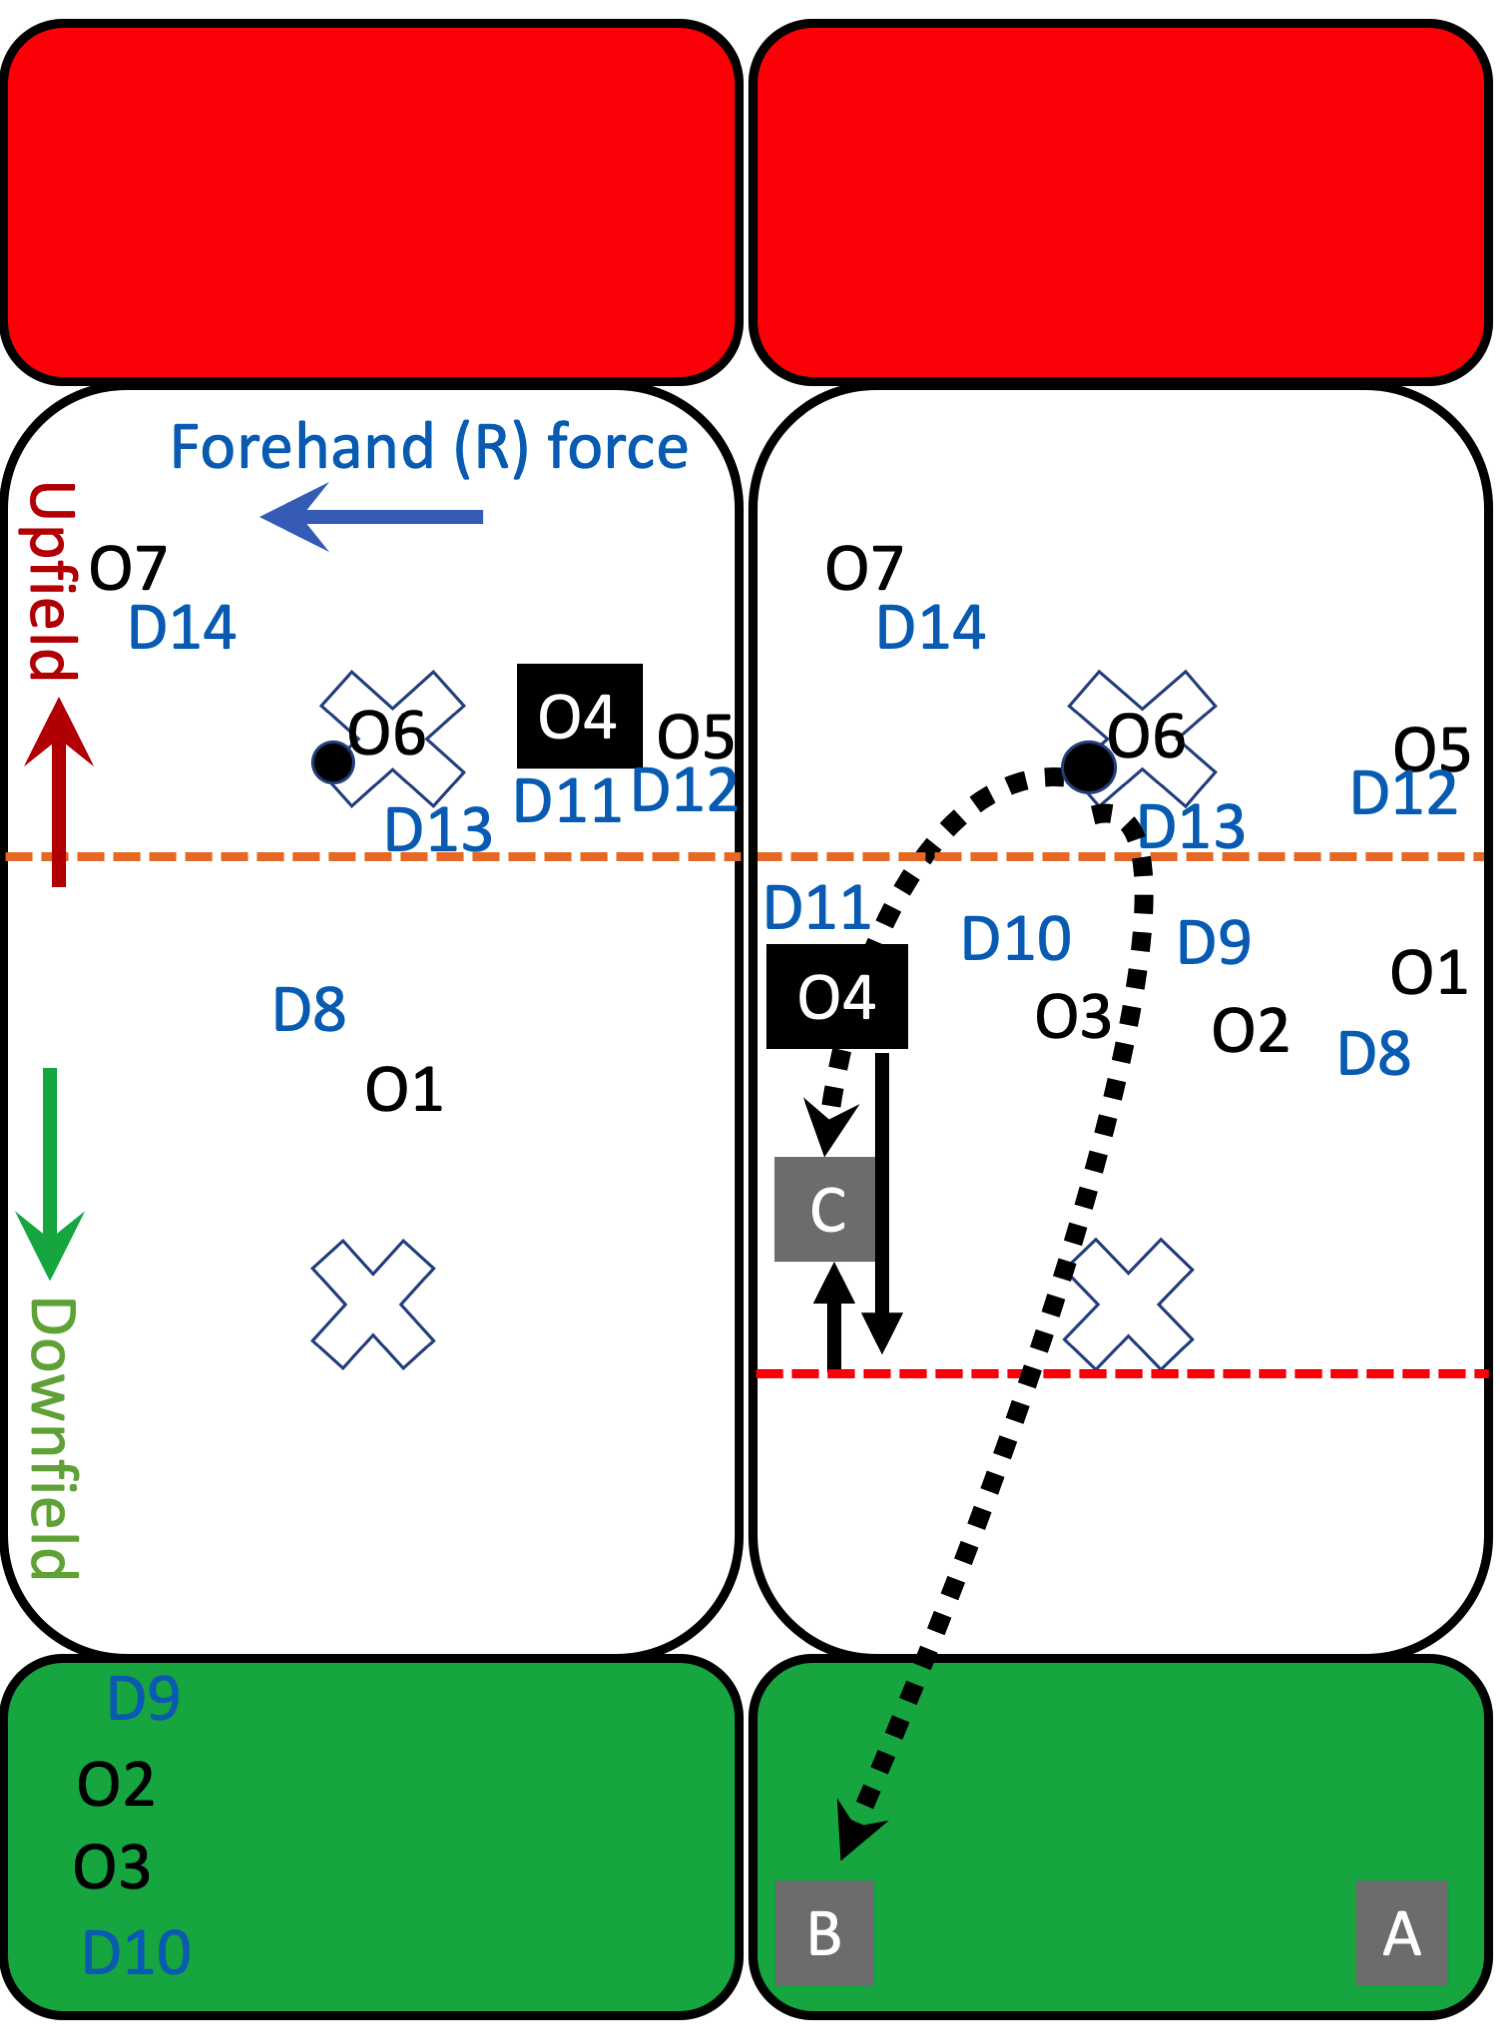
\includegraphics[width=\linewidth]{O4-horizontal}
  \caption{Feld (left) \& ho-ro (right)}
  \label{fig:O4-horizontal}
\end{marginfigure}

It may be that 
one of 
D9 
and D10 
go to help D8 
cover D1.  
If so, 
you and O2 
might spread out, 
one on each side line,
and move a bit closer, 
so as to receive a pass from 
the handlers directly.  


\subsection{Beating person-match defence with a horizontal stack}\label{sec:horizontall}
Horizontal stack 
typically involves cutting
upfield and downfield (black arrows)
within your quarter of the field\footnote{
Other cuts
can work, 
but might need
communication,
e.g. diamond cuts 
involve trading places 
with O1 
or O4.}
as shown in 
Figure \ref{fig:O4-horizontal}(right).
O6 
can potentially 
throw to you 
in the endzone 
or at C\footnote{
Black arrows
show how a back-under cut 
opens space 
for the throw 
to C.}. 

\section{Beating zone defence}\label{sec:zone}
\begin{marginfigure}%
  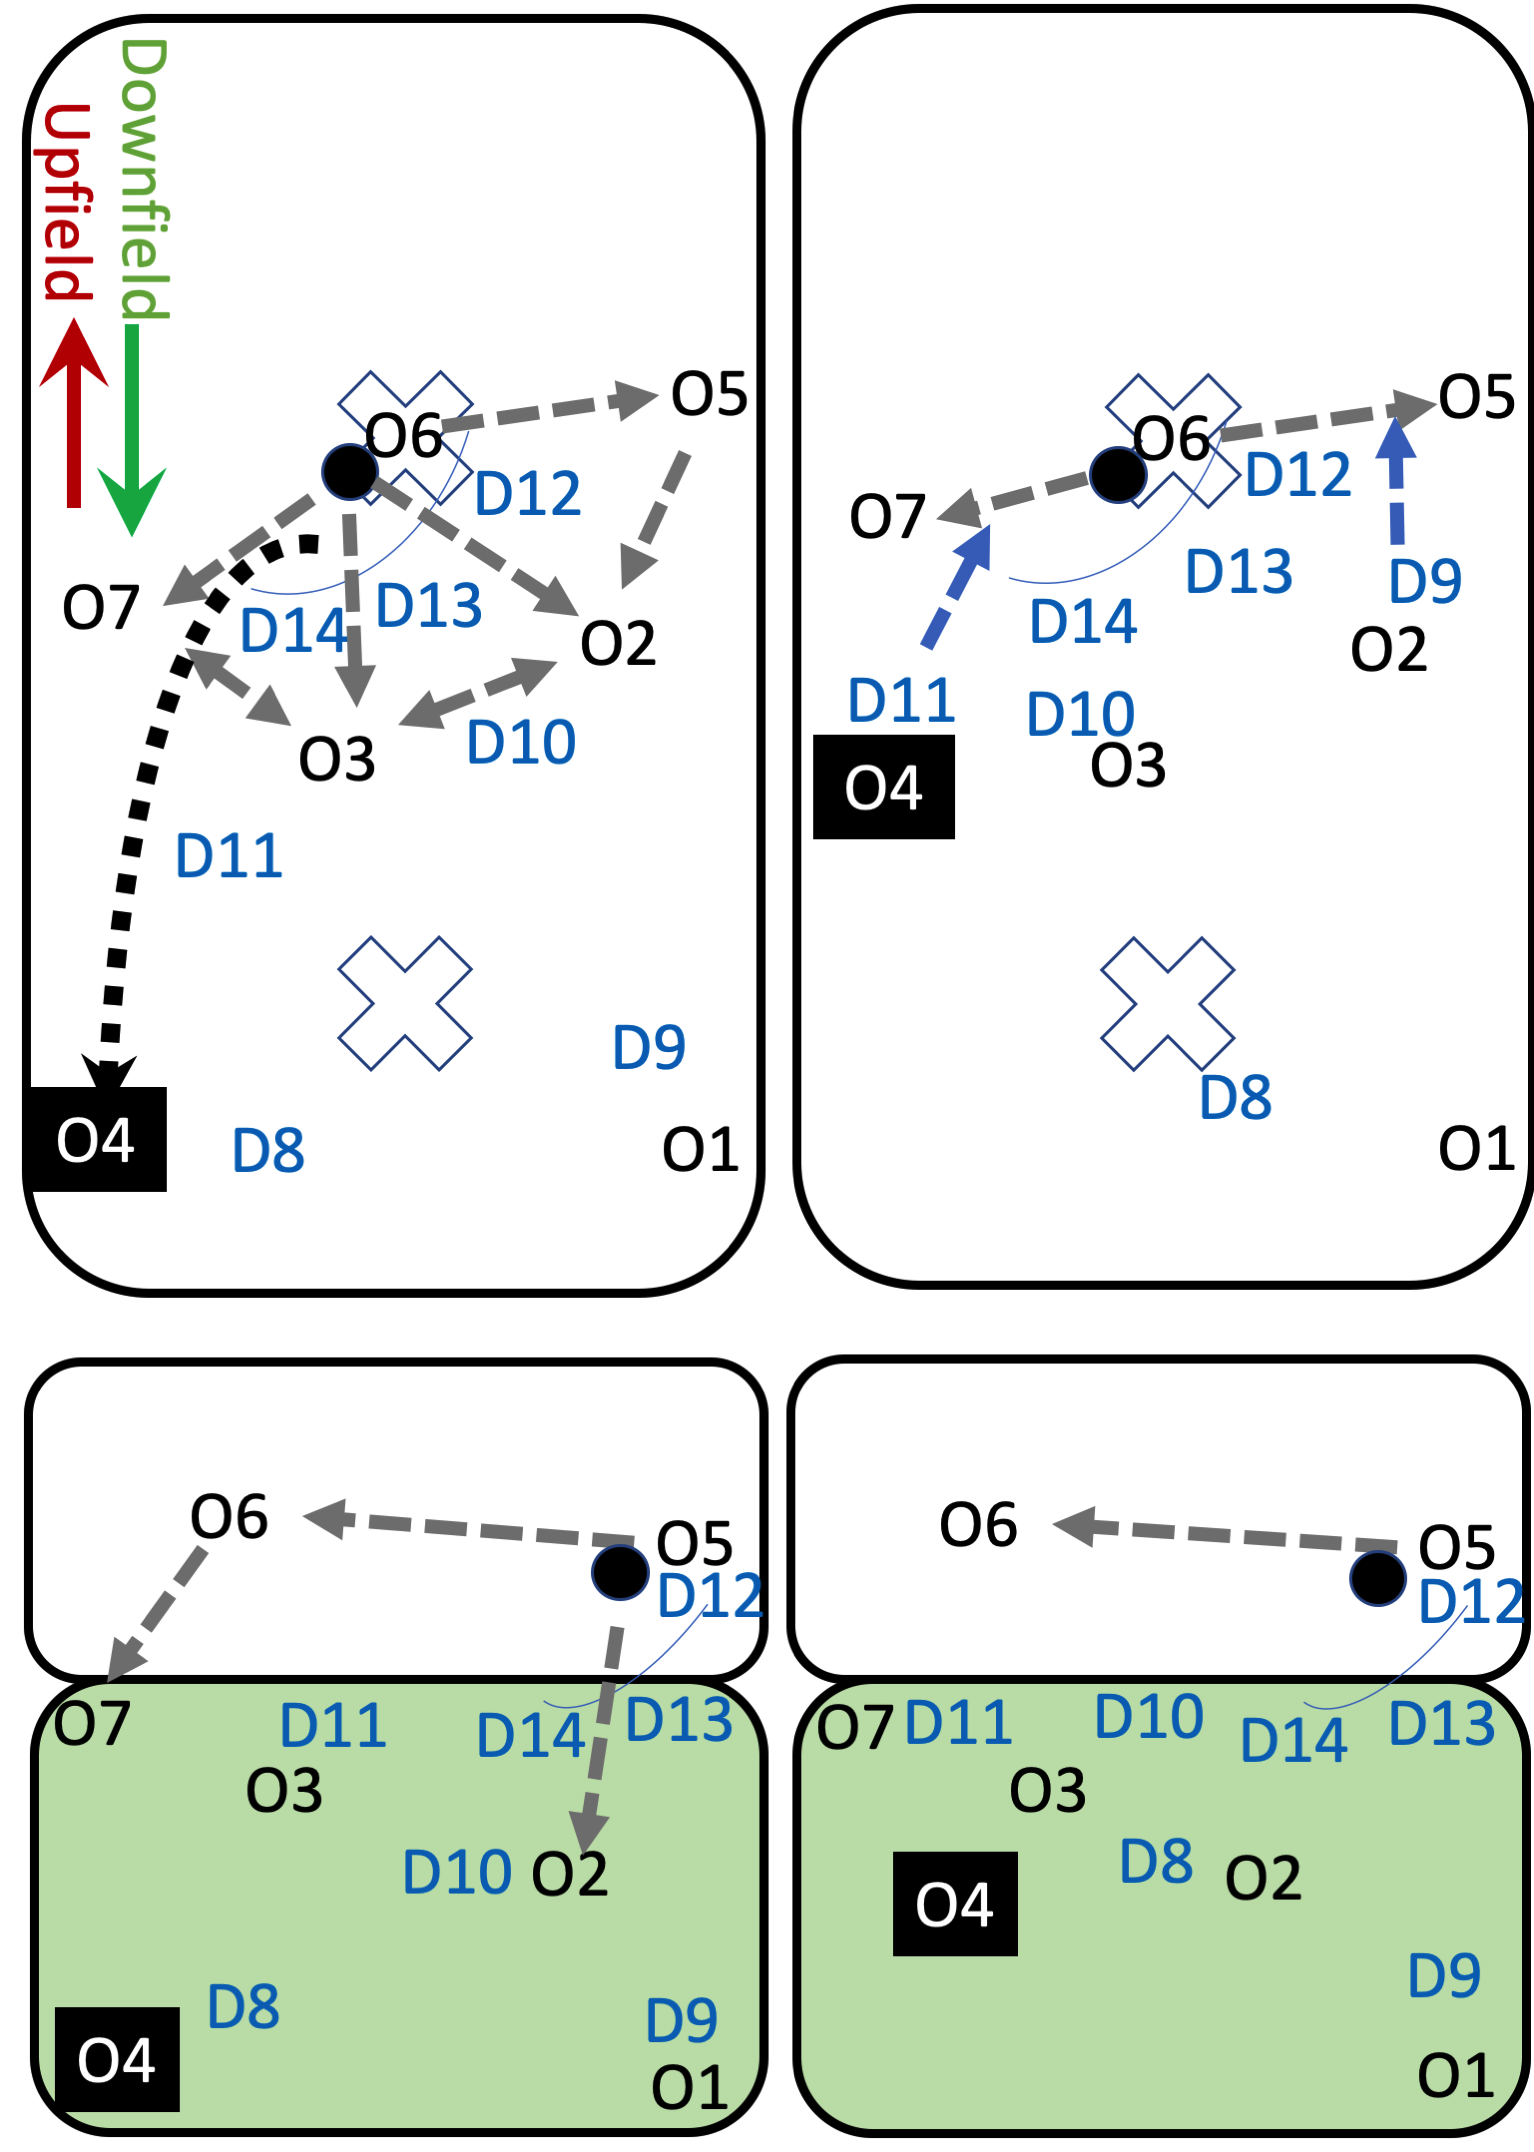
\includegraphics[width=\linewidth]{O4-zone331}
  \caption{formations against 331 zone}
  \label{fig:O4-zone331}
\end{marginfigure}
Vertical stack 
probably won't work
against zone. 
Instead, your 
team might do better spreading out, 
as shown 
in Figure \ref{fig:O4-zone331}. 
Three ways to beat a zone are:
(1) over;
(2) round; or
(3) through. 
Figure \ref{fig:O4-zone331}
(top left)
shows this 
with you 
behind the cup, 
potentially receiving a pass 
\smallcaps{through} 
between 
D13 
and D14, or 
\smallcaps{over} 
the cup\footnote{
Short hammer, scoober.}.
Alternatively, 
it might go 
\smallcaps{round} 
to O7 then 
\smallcaps{further round} to you.

Also to consider
is how you 
coordinate 
with O2 
to split 
D10. 
Figure \ref{fig:O4-zone331}
(top left), 
shows D10 
having to 
cover both 
you and O2, 
maybe with help 
from D9 
and D11. 
In contrast, 
Figure \ref{fig:O4-zone331}
(top right) 
shows a position 
that might occur 
if you `crash' 
the cup\footnote{ 
Crashing 
might  
disrupt the 
cup's formation and 
allow a stall reset.  
But, I'm not a huge fan, 
unless its a handlers 
crashing from behind, 
because you lose 
a player downfield},
which allows
D10 
to ignore you 
and play 
tighter on O2\footnote{ 
It might also allow 
D11 to threaten to intercept 
a pass to O7, 
and the rest of the cup 
(D12-13) 
to do more 
to block throws 
to O2 or O5. 
In general, 
crashing the cup
changes 
the downfield situation 
to 3 (O1, O2 and O4) 
versus 4 (D8-11), 
which is not ideal.}. 
Figure \ref{fig:O4-zone331}hat
(bottom left and right)
show two possible 
positions close to the 
endzone. 
Again, as O4
your role might 
be to try 
and work with 
O2, O5 and O7 
such that D10 
and D11 are unable to 
cover you all.   


\section{Beating clam defence}\label{sec:zone}
Clam mixes person-match 
and zone defence styles, 
with defenders 
switching frequently.
%\footnote{
%For example, 
%in Figure \ref{fig:O4-vertical}(left) 
%D8 
%might cover 
%O1 deep, 
%switching later 
%(with D9 or D11
%to cover O4's cut deep,
%rather than following O1 
%upfield to C.}. 
You might
coordinate 
with others  
to overload 
a defender, 
or spread out 
and give the handlers 
space 
and targets deep. 

\newthought{...and finally} 
this is just a two pager; 
there are many more 
offensive strategies 
and tactics\footnote{
Try no formation, just a string: O1-throws-to-O2-who-throws-to-O4-etc. Bonus points for getting all the way to O7 before scoring!}
Remember, 
defence wins games, 
offence loses them\footnote{
Because the team with the least turnovers 
usually wins.};.
and it's better to get it back 
with another turnover\footnote{
i.e. if you offence fails, then its time to play defence, even though you're the O team :)}
than receiving another pull!

\end{document}
